% ncse_new/p2_InterpolationApproximation/ch2_PiecewisePolynomials/ex_QuadraticSplines.tex
% exercise requires:   quadspline_p.p
% solutions require:   quadspline.m  ex_QuadraticSplinesPlot.m  interpol_quad_T2.eps  ex_QuadraticSplinesConv.m  time-error_QuadSplines.eps


\begin{problem}[Quadratic Splines \coreproblem] \label{prb:QuadraticSplines}

\lref{def:spline} introduces spline spaces $\Cs_{d,\Cm}$ of any degree
{$d\in\bbN_{0}$} on a node set $\Cm\subset\bbR$. \lref{sec:csi} discusses
interpolation by means of cubic splines, which is the most important case.
In this problem we practise spline interpolation for quadratic splines
in order to understand the general principles.

Consider a 1-periodic function $f: \mathbb{R} \rightarrow \mathbb{R}$, that is,
$f(t+1)=f(t)$ for all $t\in\bbR$, and a set of nodes
\begin{gather*}%    \label{eq:2}
\mathcal{M}:=\{0=t_0<t_{1}<t_{2}<\dots<t_{n-1}<t_n=1\}\subset[0,1]\;.
\end{gather*}
We want to approximate $f$ using a \emph{1-periodic} quadratic spline function
$s\in\Cs_{2,\Cm}$, which interpolates $f$ \emph{in the midpoints} of the intervals
$[t_{j-1},t_{j}]$, $j=0,\ldots,n$.

In analogy to the local representation of a cubic spline function according to
\lref{cs:rep}, we parametrize a quadratic spline function
$s\in\mathcal{S}_{2,\Cm}$ according to
\begin{gather} \label{eq:quad_spl}
s|_{[t_{j-1},t_{j}]}(t) = d_{j}\;\tau^{2} + c_{j}\;4\;\tau(1-\tau) + d_{j-1}\;(1-\tau)^{2}\;,
\quad \tau := \frac{t-t_{j-1}}{t_{j}-t_{j-1}}\;,\quad
j=1,\ldots,n\;,
\end{gather}
with $c_j,d_k\in\bbR$, $j=1,\ldots,n,\; k=0,\ldots,n$.
Notice that the coefficients $d_k$ are associated with the nodes $t_k$ while the $c_j$ are associated with the midpoints of the intervals $[t_{j-1},t_j]$.


% ================= SUBPROBLEM 1

\begin{subproblem}[1] \label{subprb:QuadraticSplines_1}
What is the dimension of the subspace of \emph{1-periodic} spline functions in $\Cs_{2,\Cm}$?

\begin{solution} Counting argument, similar to that used to determine the
  dimensions of the spline spaces. We have $n+1$ unknowns $d_k$ and $n$ unknowns
  $c_j$, the constraint $d_0=s(t_0) = s(t_0+1) = s(t_n) = d_n$ leaves us with a
  total of $2n$ unknowns.  The continuity of the derivatives in the $n$ nodes
  impose the same number of constraints, therefore the total dimension of the
  spline space is $2n-n=n$.
\end{solution}
\end{subproblem}

% ================= SUBPROBLEM 2

\begin{subproblem}[1]  \label{subprb:QuadraticSplines_2}
What kind of continuity is already guaranteed by the use of the representation \eqref{eq:quad_spl}?

% need more explanations: student from last year assumed that C_1 is guaranteed since we _enforce_ it...

\begin{solution}
 We observe that $s(t_j^-)=s|_{[t_{j-1},t_{j}]}(t_j) = d_j = s|_{[t_{j},t_{j+1}]}(t_j)=s(t_j^+)$, thus we get continuity for free.
However the derivatives do not necessarily match.
\end{solution}
\end{subproblem}

% ================= SUBPROBLEM 3

\begin{subproblem}[3]  \label{subprb:QuadraticSplines_3} 
    Derive a linear system of equations (system matrix and right hand side) whose
    solution provides the coefficients $c_{j}$ and $d_{j}$ in \eqref{eq:quad_spl} from the
    function values $y_{j} := f(\frac{1}{2}(t_{j-1}+t_{j}))$, $j=1,\ldots,n$.

    \hint{} By \lref{def:spline} we know $\Cs_{2,\Cm}\subset C^{1}([0,1])$,
    which provides linear constraints at the nodes, analogous to \lref{cs:cc} for
    cubic splines.


\begin{solution}
We can plug $t = \frac{1}{2}(t_j + t_{j-1})$ into \eqref{eq:quad_spl}
and set the values equal to $y_j$. We obtain $\tau=1/2$ and the following conditions:
\begin{equation}\label{matching_y}
 \frac{1}{4} d_j + c_j + \frac{1}{4} d_{j-1} = y_j,\quad j=1,...,n.
\end{equation}
We obtain conditions on $d_j$ by matching the derivatives at the interfaces.
The derivative of the quadratic spline can be computed from \eqref{eq:quad_spl}, after defining $\Delta_j=t_j-t_{j-1}$:
$$s'|_{[t_{j-1},t_{j}]}(t)=\Delta_j^{-1}\frac{\partial}{\partial \tau}\Big( \tau^{2}d_{j} + 4\tau(1-\tau)c_{j} + (1-\tau)^{2}d_{j-1}\Big)
=\Delta_j^{-1}\Big(2\tau d_j+4(1-2\tau)c_j-2(1-\tau)d_{j-1}\Big).$$
Setting $\tau=1$ in $[t_{j-1},t_j]$ and  $\tau=0$ in $[t_j,t_{j+1}]$,
the continuity of the derivative in the node $t_j$ enforces the condition
$$\frac{2d_j-4c_j}{\Delta_j}
= s'|_{[t_{j-1},t_{j}]}(t_j)
= s'(t_j^-) = s'(t_j^+)
= s'|_{[t_{j-1},t_{j}]}(t_j)
= \frac{4c_{j+1}-2d_j}{\Delta_{j+1}}; $$
(this formula holds for $j=1,\ldots,n$ if we define $t_{n+1}=t_1+1$ and $c_{n+1}=c_1$).
Simplifying for $d_j$ we obtain:
\begin{align*}
d_j & = \frac{2\frac{c_j}{\Delta_j}+2\frac{c_{j+1}}{\Delta_{j+1}}}{\frac1{\Delta_j}+\frac1{\Delta_{j+1}}}
      = 2\frac{c_j\Delta_{j+1}+c_{j+1}\Delta_j}{\Delta_j+\Delta_{j+1}}
      = 2\frac{c_j(t_{j+1}-t_j)+c_{j+1}(t_j-t_{j-1})}{t_{j+1}-t_{j-1}},\qquad j=1,\ldots,n.
\end{align*}
Plugging this expression into \eqref{matching_y}, we get the following system of equations:
\begin{equation}\label{sys_eq_c_full}
\frac{1}{2}\frac{c_{j+1}(t_{j}-t_{j-1}) + c_j(t_{j+1}-t_j)}{t_{j+1}-t_{j-1}}
+ c_j + \frac{1}{2}\frac{c_{j}(t_{j-1}-t_{j-2}) + c_{j-1}(t_{j}-t_{j-1})}{t_{j}-t_{j-2}} = y_j,\qquad j=1,\ldots,n,
\end{equation}
with the periodic definitions $t_{-2} = t_{n-2}-1$, $c_0 = c_n$, $c_{-1} = c_{n-1}$.
We collect the coefficients and finally we obtain
\begin{equation}\label{simplif_eq_c}
\underbrace{\left\{\frac{1}{2} \frac{t_j-t_{j-1}}{t_j-t_{j-2}}\right\}}_{A_{j-1}} c_{j-1} +
\underbrace{\left\{\frac{1}{2} \frac{t_{j+1}-t_{j}}{t_{j+1}-t_{j-1}} + 1
  + \frac{1}{2} \frac{t_{j-1}-t_{j-2}}{t_{j}-t_{j-2}}\right\}}_{B_{j}} c_{j}
+ \underbrace{\left\{\frac{1}{2} \frac{t_j-t_{j-1}}{t_{j+1}-t_{j-1}}\right\}}_{C_{j+1}} c_{j+1} = y_j,\quad j=1,\ldots,n.
\end{equation}
If we have an equidistant grid with $t_j - t_{j-1} = 1/n$, this simplifies to
\begin{equation*}%\label{equi_simpl_eq_c}
 \frac{1}{4}c_{j-1} + \frac{3}{2} c_j + \frac{1}{4} c_{j+1} = y_j,\qquad \qquad j=1,\ldots,n.
\end{equation*}
The system of equations in matrix form looks as follows:
\begin{equation}\label{system}
 \begin{pmatrix}
  B_1 & C_2 & 0 & 0 & 0 & \cdots \cdots & 0 & 0 & 0 & A_0\\
  A_1 & B_2 & C_3 & 0 & 0 & \cdots \cdots & 0 & 0 & 0 & 0 \\
  0 & A_2 & B_3 & C_4 & 0 & \cdots \cdots & 0 & 0 & 0 & 0 \\
  \vdots & \vdots & \ddots & \ddots & \ddots &  & \vdots & \vdots & \vdots & \vdots \\
  \vdots & \vdots & \vdots & \ddots & \ddots & \ddots & \vdots & \vdots & \vdots & \vdots \\
  \vdots & \vdots & \vdots & \vdots & \ddots & \ddots & \ddots & \vdots & \vdots & \vdots \\
  \vdots & \vdots & \vdots & \vdots & \vdots& \ddots & \ddots & \ddots & \vdots & \vdots \\
  \vdots & \vdots & \vdots & \vdots & \vdots & & \ddots & \ddots & \ddots & 0 \\
  0 & 0 & 0 & 0 & 0 & \cdots \cdots & 0 & A_{n-2} & B_{n-1} & C_n \\
  C_{n+1} & 0 & 0 & 0 & 0 & \cdots \cdots & 0 & 0 & A_{n-1} & B_n \\
 \end{pmatrix}
 \begin{pmatrix}c_1\\c_2\\c_3\\\vdots\\\vdots\\\vdots\\\vdots\\\vdots\\c_{n-1}\\c_n\end{pmatrix}
=\begin{pmatrix}y_1\\y_2\\y_3\\\vdots\\\vdots\\\vdots\\\vdots\\\vdots\\y_{n-1}\\y_n\end{pmatrix}.
\end{equation}
\end{solution}
\end{subproblem}

% ================= SUBPROBLEM 4

\begin{subproblem}[3]  \label{subprb:QuadraticSplines_4}
Implement an \emph{efficient} \Matlab{} routine
\begin{center}
  \texttt{function s=quadspline(t,y,x)}
\end{center}
which takes as input
a (sorted) node vector \texttt{t} (of length $n-1$, because $t_{0}=0$ and $t_{n}=1$ will be taken for granted),
a $n$-vector \texttt{y} containing the values of a function $f$ at the midpoints $\frac{1}{2}(t_{j-1}+t_{j})$, $j=1,\ldots,n$,
and a \emph{sorted} $N$-vector \texttt{x} of evaluation points in $[0,1]$.

The function is to return the values of the interpolating quadratic spline $s$ at
the positions \texttt{x}.

You can test your code with the one provided by \texttt{quadspline\_p.p} (available on the lecture website).

\begin{solution}
See \autoref{mc:quadspline}.
\lstinputlisting[caption={Construction of the quadratic spline and evaluation.},label={mc:quadspline}, escapechar={}]
{\problems/ch_piecewisepolynomials/MATLAB/quadspline_better.m}

It is important not to get lost in the indexing of the vectors. In this code they can be represented as:\\
{\tt t=(t1, t2, ..., t\{n-1\})} \quad length $=n-1$,\\
{\tt ext\_t=(t\{n-1\}-1, t0=0, t1, t2,..., t\{n-1\}, tn=1, 1+t1)}\quad length $=n+3$,\\
{\tt de\_t=(1-t\{n-1\}, t1, t2-t1,..., t\{n-1\}-t\{n-2\}, 1-t\{n-1\}, t1)}\;,\\
{\tt dde\_t=(t1+1-t\{n-1\}, t2, t3-t1,..., 1-t\{n-2\}, t1+1-t\{n-1\})}\;.\\
The vectors \texttt{A,B,C,c,d} have length $n$ and correspond to the definitions given in \ref{subprb:QuadraticSplines_3} (with the indexing from 1 to $n$).
\end{solution}
\end{subproblem}

% ================= SUBPROBLEM 5

\begin{subproblem}[1] \label{subprb:QuadraticSplines_5} Plot $f$ and the
  interpolating periodic quadratic spline $s$ for $f(t) := \exp(\sin(2\pi t))$,
  $n=10$ and $\Cm = \left\{\frac{j}{n}\right\}_{j=0}^{10}$, that is, the spline is
  to fulfill $s(t)=f(t)$ for all midpoints $t$ of knot intervals.

\begin{solution}See code \ref{mc:quadspline_plot} and Figure \ref{fig:interpol_quad_T2}.
\lstinputlisting[caption={Plot of the quadratic splines.},label={mc:quadspline_plot}, escapechar={}]
{\problems/ch_piecewisepolynomials/MATLAB/ex_QuadraticSplinesPlot.m}
\begin{figure}[htb]
\caption{Quadratic spline interpolation of $f$ in 10 equispaced nodes.}\label{fig:interpol_quad_T2}
\centering 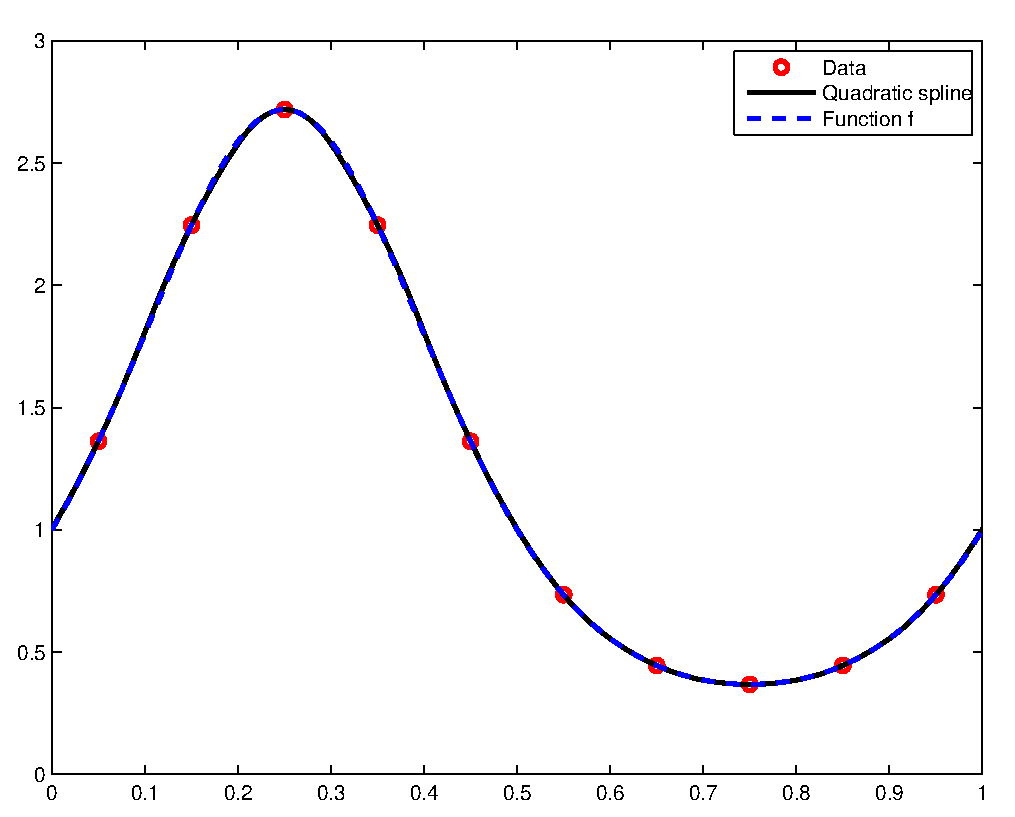
\includegraphics[width = 0.6 \textwidth]{\problems/ch_piecewisepolynomials/PICTURES/interpol_quad_T2.eps}
\end{figure}
\end{solution}
\end{subproblem}

% \subproblem\label{subprb:QuadraticSplines_7}
% What is the asymptotic complexity of your implementation of \texttt{quadspline}
% for \emph{fixed} $n$ and $N\to\infty$?
%
% \begin{solution}The evaluation is $\mathcal{O}(N)$.}

% ================= SUBPROBLEM 6

\begin{subproblem}[1]  \label{subprb:QuadraticSplines_6}
What is the complexity of the algorithm in \ref{subprb:QuadraticSplines_4} in dependance of $n$ and $N$?

\begin{solution}
The complexity is linear both in $N$ (sequential evaluation in different points) and in $n$, provided one exploits the sparse structure of the system and uses a rank-one modification to reduce the system to the inversion of a (strictly diagonally dominant) tridiagonal matrix.
% You can see the difference in the timing if you set \texttt{M} as dense in code~\ref{mc:quadspline}.
% For the implementation see code~\ref{mc:quadspline_conv} and Figure~\ref{fig:time-error_QuadSplines}.
% %
% \lstinputlisting[caption={Error and timing for quadratic splines.},label={mc:quadspline_conv}, escapechar={}]
% {\problems/ch_piecewisepolynomials/MATLAB/ex_QuadraticSplinesConv.m}
% %
\begin{figure}[htb]
\caption{Error and timing for quadratic splines in equispaced nodes.}\label{fig:time-error_QuadSplines}
\centering \includegraphics[width = 0.8 \textwidth]{\problems/ch_piecewisepolynomials/PICTURES/time-error_QuadSplines.eps}
\end{figure}
\end{solution}
\end{subproblem}
\end{problem}

% ================= SUBPROBLEM 7

%\subproblem \label{subprb:QuadraticSplines_7} \difficulty{1} \pts{1}
%Compute the approximation error in $L^\infty([0,1])$ norm:
% $$\N{f-s_{n}}_{L^{\infty}([0,1])} = \sup_{x\in[0,1]}|f(x)-s_n(x)|\;,$$
%where $s_{n}$ is the interpolating quadratic spline for $f$ on the equidistant node set $\Cm_{n} = \{j/n\}_{j=0}^{n}$.
%
%How is the dependence of the error on the number of subintervals $n$? Plot it.
%
%\hint: to approximate the $L^\infty$ norm you can evaluate the difference $|f(x)-s_{n}(x)|$ at $N\gg n$ equidistant points in $[0,1]$ and then take the maximum. You may choose $N=10.000$.
%
%\begin{solution}
%The error depends on $n$ as $O(n^{-3})$.
%
%\lstinputlisting[caption={Error and timing for quadratic splines.},label={mc:quadspline_conv}, escapechar={}]
%{p2_InterpolationApproximation/ch2_PiecewisePolynomials/MATLAB/ex_QuadraticSplinesConv.m}
%\begin{figure}[htb]
%\caption{Error and timing for quadratic splines in equispaced nodes.}\label{fig:time-error_QuadSplines}
%\centering \includegraphics[width = 0.8 \textwidth]{time-error_QuadSplines}
%\end{figure}
%}
